\documentclass{article}
\usepackage{amsmath}
\usepackage{graphicx}
\usepackage{float}
\usepackage{blindtext}
\usepackage[T1]{fontenc}
\usepackage[utf8]{inputenc}
\usepackage{algorithm}
\usepackage{algorithmic}

\begin{document}
Un algorithme génétique est une métaheuristique évolutionnaire à l'origine proposée par Holland [1]. Depuis lors, il est devenu une méthode puissante pour résoudre de nombreux problèmes d'optimisation combinatoire difficiles, dont la liste peut être trouvée dans de nombreuses références, voir par exemple [2]. Les étapes générales de l'algorithme peuvent être décrites comme suit:
\newline

\begin{algorithm}[H]
	\caption{Algorithme génétique}
	\begin{algorithmic}
		\STATE Générer une population initiale\;
		\WHILE{le critère d'arret n'est pas encore rencontré}
			\STATE Choisir des paires pour la reproduction\;
			\STATE Effectuer des croisements pour générer des descendants\;
			\STATE Faire des fluctuations dans les nouveaux descendants (mutation)\;
			\STATE Evaluer l'aptitude de nouveaux descendants\;
			\STATE Générer une nouvelle population\;
		\ENDWHILE
	\end{algorithmic}
\end{algorithm}

Un élément clé de l'AG est la génération d'une population dont les composants sont appelés \textit{chromosomes}, un terme emprunté à la génétique. Un \textit{chromosome} est en fait une représentation codée d'une solution; dont chaque composant est appelé \textit{gène}

\section{Algorithme Génétique}
On représente une solution du Bin packing comme suit : 
\begin{itemize}
	\item On a \textbf{n} articles à ranger donc on utilisera n boîtes au pire des cas (un objet par boite).
	\item On suppose que chaque boîte est composée de \textbf{n} cellules, où chaque cellule ne peut contenir qu’un seul article.
	\item Chaque cellule à un numéro unique dans la solution.
	\item Si la cellule de l’ordre \textbf{i} de la boite \textbf{j} est remplie par un objet, alors on aura plus le droit de ranger un objet dans toutes les cellules de l’ordre \textbf{i} des autres boites.
	\item La cellule \textbf{zero} contient le nombre de boîtes utilisées dans cette solution.
\end{itemize}
Pour décrire cette représentation, considérons l'exemple suivant. Supposons que nous ayons quatre objets (n=4) de poids 2 , 2 , 4 et 4 respectivement, affectés à trois boîtes  (c0=3)  comme indiqué ci-dessous :
\begin{figure}[H]
  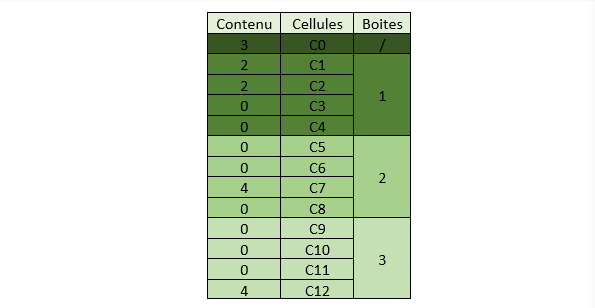
\includegraphics[width=\linewidth]{../figures/pic01.PNG}
\end{figure}
Avec c0 : contient le nombre de boîtes utilisées.
\newline
Le chromosome correspondant peut être défini comme suit:
\begin{figure}[H]
  
\includegraphics[width=\linewidth]{../figures/pic02.PNG}
\end{figure}
Cependant, avec cette représentation,les chromosomes ont une longueur égale à 1 + n² (un entier pour chaque cellule), alors pour les grands n, nous aurons besoin d'une grande quantité de mémoire pour les stocker.
Pour cela, nous utiliserons une représentation plus compacte qui utilise des chromosomes de longueur n + 1 au lieu de 1 + n². Cette dernière consiste à garder trace que des numéros des cellules remplies (ou utilisées).
\newline
Dans l'exemple ci-dessus, nous avons utilisé les cellules (c1,c2,c7,c12) et la cellule c0, nous aurions donc la séquence 
\begin{figure}[H]
  
\includegraphics[width=\linewidth]{../figures/pic03.PNG}
\end{figure}
qui a une longueur de n + 1, avec n = 4. 
\newline
\newline
Dans la première cellule, cellule 0, on stocke le nombre de boîtes utilisées qui est de 3 boites. Les numéros suivants indiquent les numéros de cellules dans lesquels les objets sont placés.
\newline
\newline
\textbf{Récupérer la solution depuis un chromosome: }
\begin{enumerate}
	\item Le nombre de boîtes utilisées est obtenu à partir de la cellule 0. 
	\item Pour obtenir dans quelle boîte chaque article a été affecté, on suit les étapes suivantes: 
	\begin{itemize}
		\item On pose c le numéro de la cellule et n le nombre d’articles
		\item On calcule : a= c mod (n) et b=[c/n] où c = bn + a
		\item  Si a=0  (c est divisible par n), alors: 
		\begin{itemize}
			\item Le numéro de l’article est\textbf{ sa position dans le chromosome} et le numéro de la boîte où il est rangé  est \textbf{b}.
		\end{itemize}
		Sinon:
		\begin{itemize}
			\item Le numéro de l’article est \textbf{sa position dans le chromosome} et le numéro de la boîte où il est rangé est \textbf{1 + b}.
		\end{itemize}
	\end{itemize}
\end{enumerate}
Dans l'exemple ci-dessus, pour la cellule 7, nous avons: 7 = 1 × 4 + 3, 
le reste est a= 3 et b = 1, donc b + 1 = 2, donc l'objet 3 est placé dans la boîte 2. 
Pour la cellule 12, nous avons: 12 = 3 × 4 + 0, le reste est a= 0, et b = 3, donc l'objet 4 est placé dans la boîte 3
\subsection{Initialisation}
La génération de la population initiale en :
		\begin{itemize}
			\item Changeant l’ordre des objets aléatoirement.
			\item Génération du chromosome avec \textbf{First Fit}
		\end{itemize}
\subsection{Selection (Choix d'une paire pour la reproduction)}
C’est la phase qui consiste à choisir les individus à reproduire et ceux qui participent à la construction d’une nouvelle population. Nous avons opté pour la méthode du Tournament Selection.
\subsection{Tournament Selection}
Dans cette approche, un "tournoi, k" est organisé entre k chromosomes (solutions)choisis au hasard dans la population et celui avec la meilleure forme physique (Fitness Value) est sélectionné comme gagnant et sera autorisé à se reproduire.
\newline
Supposons que k = 3 :
\begin{figure}[H]
  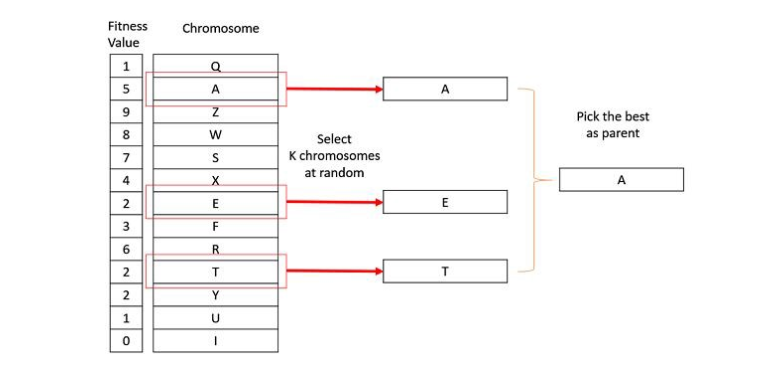
\includegraphics[width=\linewidth]{../figures/pic04.PNG}
\end{figure}
La pression de sélection(Une \textit{pression de sélection} est une contrainte environnementale qui va \textbf{pousser} une espèce à évoluer dans une direction donnée.) peut être facilement ajustée en changeant la taille du tournoi (un k plus élevé augmente la pression de sélection).
La sélection du tournoi est indépendante de la fonction Fitness.Parmis ces avantages, on cite la diminution le temps de calcul, et son fonctionnement sur les architectures parallèles.
\subsection{Croisement}
L'opérateur de croisement est analogue à la reproduction et au croisement biologique. Dans ce cas, plus d'un parent est sélectionné et un ou plusieurs descendants sont produits en utilisant le matériel génétique des parents. Le crossover est généralement appliqué dans une AG à forte probabilité \textit{pc}
\newline
L’opérateur choisi pour cet algorithme est le ‘One Point Crossover’ ou ‘le croisement à un point’. Dans ce croisement, un point de croisement aléatoire est sélectionné et les queues de ses deux parents sont échangées pour obtenir de nouveaux descendants, ce qui revient à diviser l’ensemble des boîtes en deux fragments et échanger les objets de ces derniers.
\newline
Par exemple dans la figure suivante, nous avons le point de croisement =5:
\begin{figure}[H]
  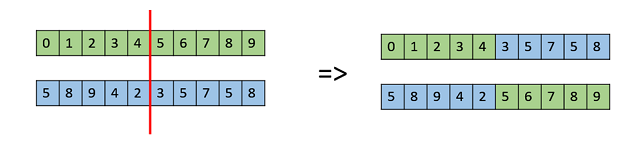
\includegraphics[width=\linewidth]{../figures/pic05.PNG}
\end{figure}
\subsection{Mutation}
La mutation peut être définie comme un petit ajustement aléatoire dans le chromosome, pour obtenir une nouvelle solution. Il est utilisé pour maintenir et introduire la diversité dans la population génétique et est généralement appliqué avec une faible probabilité \textit{pm}. Si la probabilité est très élevée, l'AG se réduit à une recherche aléatoire.
\newline
La mutation est la partie de l'AG qui est liée à «\textbf{l'exploration}» de l'espace de recherche. Il a été observé que la mutation est essentielle à la convergence de l'AG alors que le croisement ne l'est pas.
\newline
L’opérateur de mutation choisi pour cette algorithme est :  “\textbf{scramble mutation}” ou “\textbf{la mutation de brouillage}”, qui, à partir du chromosome entier, choisit aléatoirement un sous-ensemble de gènes dont le cardinale est un paramètre en entrée de la fonction, et ses valeurs sont brouillées ou mélangées au hasard.
\begin{figure}[H]
  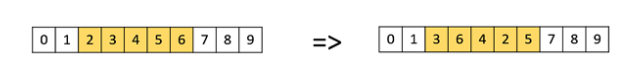
\includegraphics[width=\linewidth]{../figures/pic06.PNG}
\end{figure}
\subsection{Evaluation}
Le choix du chromosome ayant la plus petite valeur de la cellule 0, c’est à dire le plus petit nombre de boîtes après avoir vérifié la validité de la solution (chromosome) i.e si le chromosome constitue réellement une solution acceptable.
\subsection{Fitness et validation d’un chromosome}
Cette fonction nous permet de vérifier si et combien un chromosome donné est “bon” ou “fit” à notre problème. 
\newline
Pour cela il faut d’abord vérifier la validité de la solution: d’un côté vérifier si tous les articles ont effectivement été rangés dans des boîtes, et de l’autre, vérifier si le total des poids des articles dans chaque boîte est effectivement inférieur ou égal à la capacité d’une boîte. 
\newline
Après avoire effectué ces vérifications on pourra prendre comme valeur de “\textit{fitness}” du chromosome, le nombre de boîtes utilisées, stocké dans la 1ère cellule du chromosome.
\subsection{Critère d'arrêt}
L'algorithme s’arrête après un nombre d’itérations prédéfini, donné en paramètre.
\newline
\newline
\textbf{L’Algorithme AG sera à son tour exécuté plusieurs fois, selon un paramètre en entrée  ( on a opté pour 10 fois), et à la fin la solution ayant le plus petit nombre de boîtes utilisées sera prise comme solution de l’instance.}
\section{Tests}
Après avoir finalisé notre code, on a commencé la phase des tests qui a été divisée en deux partie :
\begin{enumerate}
	\item La partie des tests préliminaires.
	\item La partie des tests après le calibrage des paramètres. 
\end{enumerate}
On a utilisé pour nos tests comme instances du problème BinPacking, comme pour les méthodes précédentes (Exactes et Heuristiques), les instances du benchmark Scholl.
Les paramètres sur lesquels on a joué, sont :
\begin{itemize}
	\item \textbf{nbrGen} : le nombre de populations générées.
	\item\textbf{ k} : le paramètre de l’algorithme de sélection “\textit{le k-tournament}”
	\item \textbf{popSize} : la taille d’une population
\end{itemize}
La probabilité de croisement a été fixée  à 0.85, et la probabilité de mutation  a été fixée à son tour à 0.1.
\subsection{Les tests préliminaires}
Dans cette partie, on a voulu tester les performances de notre programme , en essayant plusieurs combinaisons des paramètres:
\begin{itemize}
	\item \textbf{nbrGen} : on a essayé 4, 50, 100, 200 et puis 500 qui lui,  ne donnait pas de meilleurs résultats que ceux obtenus avec 200 itérations.
	\item\textbf{ k} : on a essayé 4 et 25.
	\item \textbf{popSize} : on a essayé avec une population de 4 chromosomes, 8, et 10.
\end{itemize}
Au final, notre choix s’est porté sur le triplet :(\textbf{nbrGen}=200,\textbf{ k}=25,\textbf{popSize}=10) car ils donnaient d’assez bons résultats.
\subsection{Les tests après calibrage des paramètres}
Pour pouvoir confirmer notre choix de paramètres on a vu nécessaire d’utiliser un outil de calibrage, on a utilisé l'outil \textbf{IRACE}. 
\newline
Après avoir exécuté le code avec \textbf{IRACE}, on a obtenu cette combinaison des paramètres (\textbf{nbrGen}=200,\textbf{k}=25,\textbf{popSize}=10) en fixant , \textbf{probaCroisement}=0.85 et \textbf{probaMutation}=0.1, et qui est,en effet, la combinaison qui donne les meilleurs résultats dans le cas de notre programme. Ceci confirme nos résultats pour le choix des paramètres trouvés pendant les tests préliminaires.
\newline
\newline
Dans ce qui suit on présentera les résultats d’exécution de notre algorithme génétique en prenant comme paramètres ceux trouvés par l’outils \textbf{IRACE} (\textbf{nbrGen}=200,\textbf{k}=25,\textbf{popSize}=10) avec \textbf{probaCroisement}=0.85 et \textbf{probaMutation}=0.1
\newline
Voici les résultats des exécutions, pour chaque classe:
\newline
\textbf{Graphe 01:}
Graphe représentant le temps d'exécution moyen de chaque type d’instance ( la moyenne d'exécution de 5 instances de même type) des 3 classes de Scholl
\begin{figure}[H]
  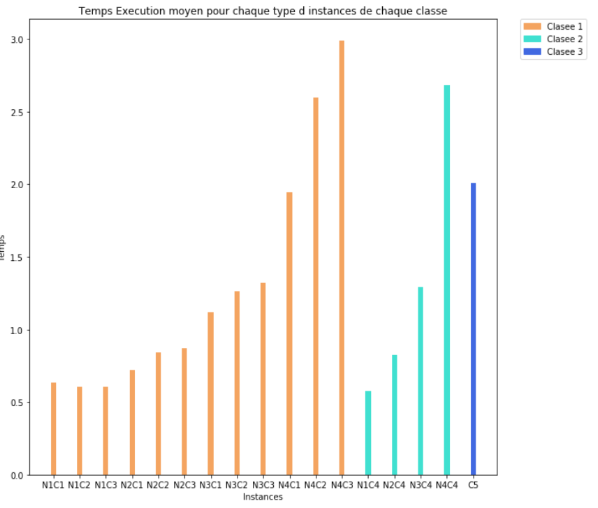
\includegraphics[width=\linewidth]{../figures/pic07.PNG}
\end{figure}
\textbf{Graphe 02:}
Les graphes suivants montrent la différence entre le nombre de boîtes utilisées par AG et  la valeur optimale OPT
\begin{figure}[H]
  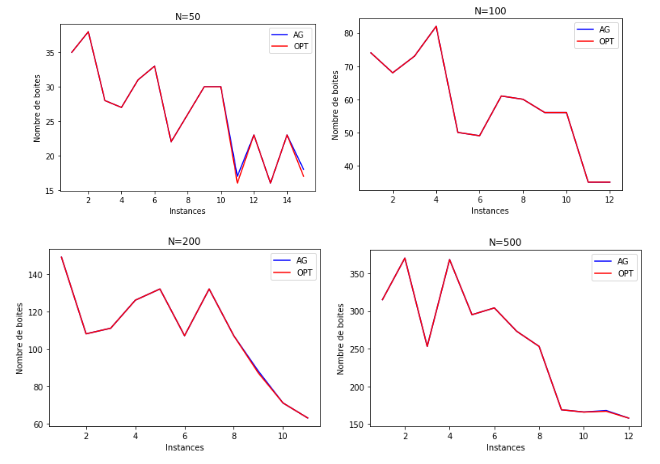
\includegraphics[width=\linewidth]{../figures/pic08.PNG}
\end{figure}
\begin{figure}[H]
  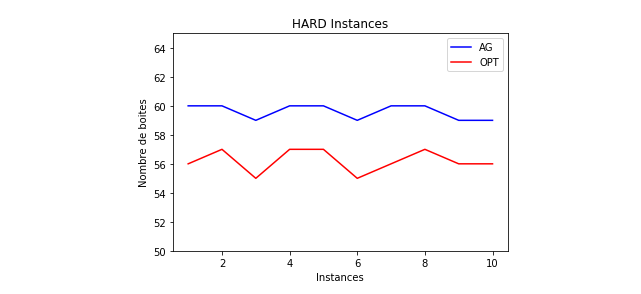
\includegraphics[width=\linewidth]{../figures/pic09.PNG}
\end{figure}
Voici les ratio obtenus par famille d’instances :
\begin{figure}[H]
  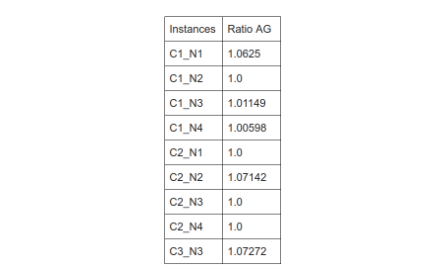
\includegraphics[width=\linewidth]{../figures/pic10.PNG}
\end{figure}
\textbf{Graphe 03:}
Et voici le graphe des ratio pour chaque nombre d'objets N des instances 
\begin{figure}[H]
  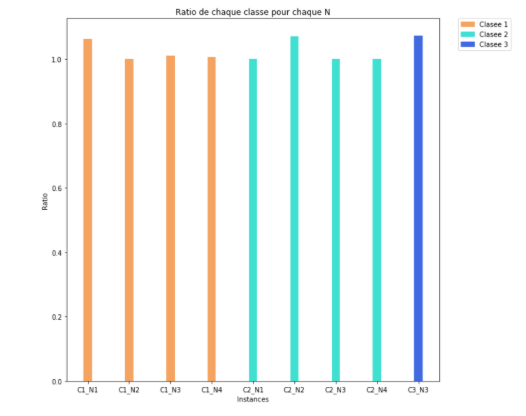
\includegraphics[width=\linewidth]{../figures/pic11.PNG}
\end{figure}
\textbf{Analyse et Interprétation des résultats : }
\newline
\begin{itemize}
	\item Le temps d’exécution correspond à dix exécutions du AG, ceci était nécessaire vu la nature stochastique de l’algorithme,  la solution initiale générée aléatoirement (le trie aléatoir de la liste des objets avant d’effectuer FF) et les facteurs liés aux méthodes de croisement et de mutation, influent sur les résultats obtenus.
	\item En terme de qualité de solution (étudiée en utilisant le ratio), l'AG donne d’assez bons résultats pour les instances du benchmark scholl, surtout dans le cas des classes 1 et 2 , où il arrive souvent à trouver la solution optimale sinon une valeur très proche de cette dernière, mais avec une qualité moindre dans le cas de la 3ème classe. \textbf{[Graphe 03] }
	\item Le Ratio obtenu par l’AG est proche de 1 (Worst case ratio<1.1 dans tous les cas). Ceci signifie que l’algorithme génétique donne une bonne qualité de résultats même dans le pire des cas (les instances les plus difficiles).\textbf{[Graphe 03] }
\end{itemize}

\end{document}